\documentclass[a4paper, russian]{article}
\pagestyle{empty}
\usepackage[T2A]{fontenc}
\usepackage[russian]{babel}
\usepackage[utf8]{inputenc}
\usepackage{pscyr}
\usepackage{graphicx}
\usepackage{amssymb}
\usepackage{amsmath}
\usepackage[left=25mm, right=1cm, top=2cm, bottom=25mm, bindingoffset=0cm]{geometry}
\usepackage{eso-pic}
\usepackage[tableposition=top]{caption}
\newcommand\BackgroundPic{%
\put(0,0){%
\parbox[b][\paperheight]{\paperwidth}{%
\vfill
\centering
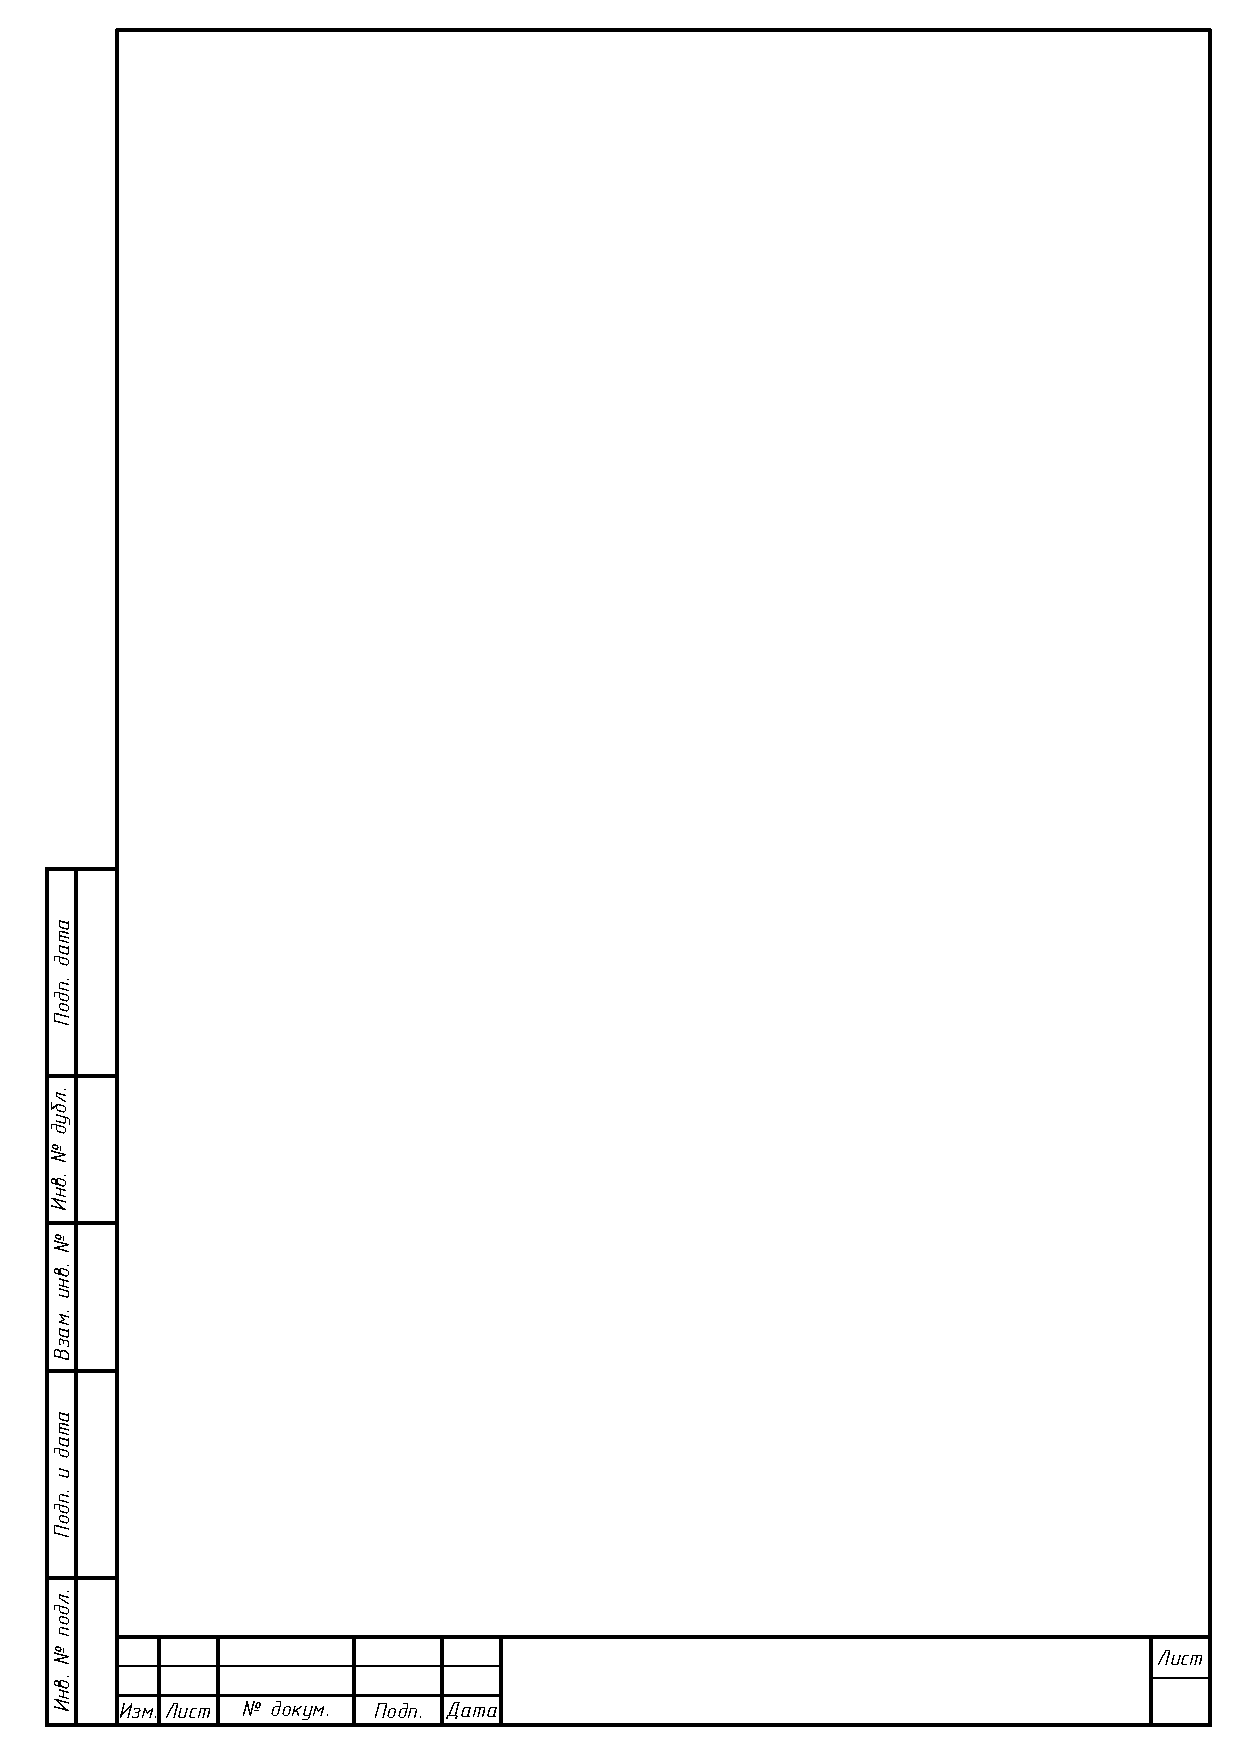
\includegraphics[%width=\paperwidth,height=\paperheight
]{Model}%
\vfill
}}}
\newcommand{\braw}{\geqslant}
\newcommand{\ruin}[1]{\text{\slshape{#1}}}
\newcommand{\knm}{\,\text{кНм}}
\frenchspacing
\AddToShipoutPicture{\BackgroundPic}
\begin{document}
Исходные данные

Прокатный цех однопролетный, пролетом 30~м, оборудован двумя мостовыми кранами грузоподъемностью $Q=32/5$~т тяжелого режима работы. Группа режима~8К. Длина здания 120~м, отметка головок рельса 9,4~м. Здание отапливаемое.

Выбрана система с шагом поперечных рам 6~м, с жестким сопряжением ригеля с колонной. Схема поперечной рамы показана на рис.\ref{shrama}
\begin{figure}
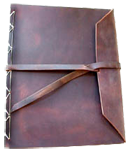
\includegraphics{007.png}
\caption{Схема поперечной рамы однопролетного здания}\label{shrama}
\end{figure}

Вертикальные размеры:

$$H_2\braw(H_k +100)+f=2750+100+350=3200\, \text{мм;}$$
Принимаем $H_2=3200$ мм:
$$H_0=H_1+H_2=9200+3200=12400\,\text{мм.}$$
При высоте подкрановой балки с рельсом, равной 1/8 ее пролета, 
$H_\ruin{в}=(h_{\text{б}}+h_{\text{р}})+H_2=600+200+3200=4000$ мм. 
При заглублении базы колонны на 600 мм ниже пола 
$H_\ruin{н}=H_0-H_\ruin{в}+600=12400-4000+600=9000$ мм. Полная высота колонн 
$H=H_\ruin{в}+H_\ruin{н}=13000$ мм; $H_\ruin{ф}=3150$ мм.

Горизонтальные размеры назначаются следующим образом. В верхней части колонн устраивается проход для осмотра крановых путей, привязка $a=500$ мм, высота сечения верхней части колонны $h_\ruin{в}=700>H_\ruin{в}/12=4000/12=333$ мм. В пределах высоты фермы высоту сечения колонны назначаем $h_\ruin{в}=700$ мм; $l_1\braw B_1+(H_\ruin{в}-a)+75=300+(700-500)+75+450=1025$ мм. Назначаем $l_1=1250$ мм (кратно 250 мм); $h_\ruin{н}=l_1+a=1250+500=1750$ мм. Пролет мостового крана 
$L_\ruin{к}=l-2l_1=30000-2\cdot1250=27500$ мм.

Сечение верхней части колонны назначаем сплошностенчатым двутавровым, нижней --- сквозным.


Расчет поперечной рамы

А. Расчетная схема рамы.

В соответствии с конструктивной схемой выбираем ее расчетную схему и основную систему. Расстояние между центрами тяжести верзнего и нижнего участков колонн
$$e_0=0.5(h_\ruin{н}-h_\ruin{в})=0.5\cdot(1750-700)=0.525\,\text{м}.$$
Соотношение моментов инерции $I_\ruin{н}/I_\ruin{в}=7; I_\ruin{р}/I_\ruin{н}=4$. Если $I_\ruin{в}=1$, то 
$I_\ruin{н}=5$. $I_\ruin{р}=20$. Сопряжение ригеля с колонной назначаем жестким (краны режима работы группы 8К, цех однопролетный).

Б. Нагрузки на поперечную раму.

Постоянная нагрузка. Нагрузка на 1 м$^2$ кровли определяем по \cite[табл. 17.3]{veden}. Расчет нагрузки в 
табл.~\ref{krov}.

\begin{table}[ht]
\caption{Постоянная нагрузка от покрытия}
\label{krov}
\centering
	\begin{tabular}{|l|p{2cm}|p{2cm}|p{2cm}|}
	\hline
		Состав покрытия & Нормативная нагрузка, кН/м$^2$ & 
		Коэффициент надежности по нагрузке & Расчетная нагрузка, кН/м$^2$ \\
	\hline
		Мембрана LOGICROOF V-RP & 0.02 & 1.3 & 0.026\\
		Мин. ватный утеплитель Техноруф В60 & 0.08 & 1.2 & 0.096\\
		Мин. ватный утеплитель Техноруф Н30 & 0.09 & 1.2 & 0.108\\
		Пароизоляция & 0.03 & 1.3 & 0.039\\
		Профилированный настил НС35-1000-0.55 & 0.06 & 1.05 & 0.063\\
		Собственный вес металлических конструкций & 0.3 & 1.05 & 0.315\\
	\hline
		& $g^\ruin{н}=0.58$ & & $g^\ruin{р}=0.65$\\
	\hline
	\end{tabular}
\end{table}

Расчетную равномерно распределенную линейную нагрузку на ригель рамы вычисляем по формуле
$$q_g=g_\ruin{кр}b_\ruin{ф}/\cos\alpha=0.65\cdot6/1=3.9\,\text{кН/м.}$$
Опорная реакция ригеля рамы $F_R=q_gl/2=3.9\cdot30/2=58.5$ кН.

Расчетный вес колонны.
По \cite[табл. 12.1]{veden} принято 0.3 кН/м$^2$. Вес верхней части (20\% веса) 
$G_\ruin{в}=1.05\cdot0.2\cdot0.3\cdot6\cdot15=5.67$ кН; вес нижней части (80\% веса)
$G_\ruin{н}=1.05\cdot0.8\cdot0.3\cdot6\cdot15=22.68$ кН.

Приняты самонесущие панели.

Снеговая нагрузка.
Вес снегового покрова $S_0=1.5$ кПа. Коэффициент надежности по нагрузке $\gamma_s=1.4.$
Линейная распределенная нагрузка от снега на ригель рамы равна
$$q_s=\gamma_sS_0b\ruin{ф}=1.4\cdot1.5\cdot6=12.6\,\text{кН/м.}$$
Опорная реакция ригеля $F_R=12.6\cdot30/2=189$ кН.

Вертикальные усилия от мостовых кранов см. на рис.
Базу крана (5.1~м), расстояние между колесами двух кранов (1.2~м), а также нормативное усилие колеса (345~кН) находим по \cite[прил.~1]{veden}. 
$$D_{max}=\gamma F \psi \Sigma F_k^n y + \gamma_g G_\ruin{пб}=
1.1 \cdot 0.95 \cdot 345 \cdot 1.9 + 1.05 \cdot 22.5 = 685 + 24 = 709\,\text{кН;}$$
(вес подкрановой балки по \cite[табл. 12.1]{veden} 
$G_\ruin{пб} = 0.25 \cdot 6 \cdot 15 = 22.5$ кН)
$${F'}_k=(Q+G_\ruin{кр})/n_0-F_k^n=(314+608)/2-345=116\,\text{кН;}$$
$$D_{min} = 685\cdot116/345+24=254\,\text{кН.}$$
Сосредоточенные моменты от вертикальных сил $D_{max}$, $D_{min}$ определяем по формуле
$$e_\ruin{к} = 0.5_\ruin{н} = 0.5 \cdot 1.75 = 0.875\,\text{м;} 
\,M_{max} = e\ruin{к} D_{max} = 0.875 \cdot 709 = 620\,\text{кНм;}$$
$$M_{min} = 0.875 \cdot 254 = 222\,\text{кНм.}$$
Горизонтальную силу от мостовых кранов находим по формулам
$$T_k^n = 0.05 (Q + G_\ruin{т}) / n_0 = 0.05 (314 + 85) / 2 = 10\,\text{кН;}$$
$$T = \gamma F \psi \Sigma T_k^n y = 1.1 \cdot 0.95 \cdot 10 \cdot 1.9 = 20\,\text{кН}$$
Считаем что сила $T$ приложена в уровне уступа колонны.

Ветровая нагрузка.
Нормативное давление ветра \cite[прил.~2]{veden} $w_0 = 0.3$ кПа. 
Тип местности Б \cite[прил.~3]{veden}, коэффициент $k$ при высоте до 5 м --- 0.5;
10 м --- 0.65 ; 20 м --- 0.85.

По формуле
$$q_w = \gamma_w w_0 k c b = 1.4 \cdot 0.3 \cdot 0.8 \cdot 6k = 2.016k.$$
Линейная распределенная нагрузка при высоте до 10 м равна $2.016 \cdot 0.65 = 1.31$
кН/м; 20 м --- $2.016 \cdot 0.85 = 1.71$ кН/м; 12.4 м --- 1.4 кН/м; 15.55 м --- 1.53 кН/м.

Сосредоточенные силы от ветровой нагрузки вычисляем по формулам:
$$F_w = (q_1 + q_2)h/2=(1.53+1.4)3.15/2=4.61\,\text{кН;}$$
$${F'}_w = F_w 0.6/0.8 = 3.46\,\text{кН,}$$
а эвкивалентные линейные нагрузки --- по формуле
$$k_\ruin{э}=0.67; \,q_\ruin{э}=q_0w_0k_\ruin{э}=2.016\cdot 0.67=1.35\,\text{кН/м;} 
\,{q'}_\ruin{э}=1.35\cdot0.6/0.8=1.01\,\text{кН/м.}$$
Ветровые нагрузки показаны на рис.

В. Статический расчет поперечной рамы.
Расчет на постоянные нагрузки. Основная система приведена на рис., а схема нагрузки --- на рис.
Сосредоточенный момент из-за смещения осей верхней и нижней частей колонны
$$M = -(F_R + F_1)e_0=-(58.5+5.67)0.525=-33.7\,\text{кНм.}$$
По \cite[табл. 12.4]{veden} находим параметры $n=1/7=0.14\approx0.15$;
$$\alpha = H_\ruin{в}/H=4/13=0.3.$$
Каноническое уравнение имеет вид $$r_{11}\varphi+r_{1p}=0.$$
Моменты от поворота узлов на угол $\varphi = 1$ равны:
$$M_A=k_Ai=0.795i;\, M_C=k_Ci=-0.341i;\, M_B=k_Bi=-0.827i;$$
$$M_B^\ruin{р}=2EI_\ruin{р}/l=2E4I_\ruin{н}H/LH=8iH/l=8\cdot13i/30=3.47i.$$
Моменты от нагрузки на стойках $M_\ruin{р}$ равны:
$$M_A=k_AM=0.344\cdot(-33.7)=-11.6\,\text{кНм;}$$
$$M_B=k_BM=-0.159\cdot(-33.7)=5.4\,\text{кНм;}$$
$$M_C^\ruin{н}=k_AM=-0.708\cdot(-33.7)=23.9\,\text{кНм;}$$
$$M_C^\ruin{в}=(k_C+1)M=(-0.708+1)\cdot(-33.7)=-9.8\,\text{кНм.}$$
Моменты на опорах ригеля (защемляемая балка постоянного по длине сечения) 
$M_B^\ruin{р}=-q_gl^2/12=-3.9\cdot30^2/12=-293$ кНм.

Определение $r_{11}$ и $r_{1p}$:
$$r_{11}=M_B+M_B^\ruin{р}=0.827i+3.47i=4.3i\,(\text{по эпюре} M_1);$$
$$r_{1p}=M_B+M_B^\ruin{р}=-5.4-293=-298\,(\text{по эпюре} M_p).$$
Угол поворота $\varphi = - r{1p}/r{11}=-298/4.3i=69.3/i$.

Моменты от фактического угла поворота ($M_1\varphi$) равны:
$$M_A=0.795i\cdot69.3/i=55.1\,\text{кНм};\,M_B=-0.827i\cdot69.3/i=-57.3\,\text{кНм};$$
$$M_C=-0.341i\cdot69.3/i=-23.6\,\text{кНм};
\,M_B^\ruin{р}=3.47i\cdot69.3/i=240.5\,\text{кНм.}$$
Эпюра моментов ($M_{1\varphi}+M_p$) от постоянной нагрузки:
$$M_A=55.1-11.6=43.5\,\text{кНм};\,M_B=-57.3+5.4=-51.9\,\text{кНм};$$
$$M_C^\ruin{н}=23.9-23.6=0.3\,\text{кНм};\,M_C^\ruin{в}=-9.8-23.6=-33.4\,\text{кНм};$$
$$M_B^\ruin{р}=240.5-292=-52.5\,\text{кНм}.$$
Проверкой правильности расчета служит равенство моментов в узле B ($52.5\approx51.9$),
равенство перепада эпюры моментов в точке C ($33.4+0.3=33.7$) внешнему моменту (33.7),
а также равенство поперечных сил на верхней и нижней частях колонны:
$$Q_{AC}=-(43.5-0.3)/9=-4.8\,\text{кН};$$
$$Q_{BC}=-(51.9-33.4)/4=-4.63\,\text{кН}.$$
Разница (3.6\%) получена в результате округления параметра $n$.
На рис. приведена эпюра нормальных сил (с учетом веса стен и собственного веса колонн).

Расчет на нагрузку от снега.
Сосредоточенный момент на колонне 
$$M=F_r e_0=-189 \cdot 0.525=-99.2\knm.$$
Моменты от нагрузки:
$$M_A=0.344(-99.2)=-34.1\knm;\, M_B=-0.159(-99.2)=15.8\knm;$$
$$M_C^\ruin{н}=-0.708(-99.2)=70.2\knm;\, M_C^\ruin{в}=0.292(-99.2)=-29\knm;$$
$$M_B^\ruin{р}=-12.6\cdot30^2/12=-945\knm.$$
Определяем $r_{11}=4.3i$; $r_{1p}=-15.8-945=-960.6$.

Угол поворота $\varphi=960.8/4.3i=223.4/i$. Моменты от фактического угла поворота:
$$M_A=0.795i\cdot223.4/i=177.6\knm;\,M_B=-0.827i\cdot223.4/i=-184.8\knm;$$
$$M_C=-0.341i\cdot223.4/i=-76.2\knm;
\,M_B^\ruin{р}=3.47i\cdot223.4/i=775.2\knm.$$
Эпюры усилий от снеговой нагрузки показаны на рис.:
$$M_A=143.5\knm; \,M_B=-169\knm; \,M_C^\ruin{в}=-105.2\knm; \,M_C^\ruin{н}=-6\knm;$$
$$M_B^\ruin{р}=-169.8\knm; \, Q_B=-(169-105)/4=-16\,\text{кН};
\,Q_A=-(143.5+6)/9=-16.6\,\text{кН};$$
$$N_B=N_A=-189\,\text{кН}; \,N_\ruin{р}=-16.6\,\text{кН}.$$

Расчет на вертикальную нагрузку от мостовых кранов при расположении крана у левой стойки.
Основная система и схема нагрузки приведены на рис.

Проверку возможности считать ригель абсолютно жестким проводим по формуле
$$k=I_\ruin{р}H/I_]ruin{н}l=28 \cdot 13 / 7 \cdot 30 = 1.73.$$
$$1.73>6/(1+1.1\sqrt{I_\ruin{н}/I_\ruin{р}-1})=6.(1+1.1\sqrt{6})=1.62$$
\begin{thebibliography}{99}
\bibitem{veden} ������������� �����������: ����� ����: ����. ��� ����� / �.�.~���������; 
��� ���. �.�.~����������.~---~7-�~���., �������. � ���. --- �.: ����������, 1998. --- 760 �.: ��.

\end{thebibliography}
\end{document}